\documentclass[a4paper, 11pt]{article}

% Pacotes Essenciais ========================================================================================================
\usepackage{lipsum}
\usepackage{titlesec}

\usepackage[utf8]{inputenc} % ................................................................. Acentuação
\usepackage[brazilian]{babel} % .................................................................. Tradução para Pt-br
\usepackage[T1]{fontenc} % .................................................................... Fontes melhores
\usepackage{graphicx} 
\usepackage[svgnames,table]{xcolor}% ................................................................ Gráficos e Cores
\usepackage{subcaption}% permite sub figuras nas imagens

\usepackage[lmargin=2.5cm,tmargin=4cm,rmargin=2cm,bmargin=3.5cm,headheight=15.1pt]{geometry} % .... Margens da ABNT
\usepackage[onehalfspacing]{setspace} % ....................................................... Espaçamento de Um e Meio
\usepackage{indentfirst} % .................................................................... Indentar o primeiro
\usepackage{enumerate} % ...................................................................... Enumeração diferenciada
\usepackage{nameref} % ........................................................................ Referência por nome
\usepackage{anyfontsize} % .................................................................... Qualquer tamanho de fonte
\usepackage{blindtext,lipsum,comment} % ....................................................... Texto cego e comentário
\usepackage{multicol,multirow} % .............................................................. Multicolunas e multilinhas
\usepackage[hidelinks]{hyperref} % ....................................................................... Links
% ===========================================================================================================================



% TikZ ======================================================================================================================
\usepackage{tikz} % ........................................................................... O completíssimo pacote TIKZ
\usetikzlibrary{calc,patterns,arrows} % ....................................................... Algumas bibliotecas do Tikz
\usepackage{pgfplots} % ....................................................................... Para usar axis no Tikz
\pgfplotsset{compat=1.17} % ................................................................... Faz o pgfplots compatível
\usepgfplotslibrary{fillbetween} % ............................................................ Preenche entre funções
% ===========================================================================================================================



% Embelezamento das páginas =================================================================================================
\usepackage{fancyhdr} % ....................................................................... Fancy é para deixar bonito
\usepackage{graphics}

\renewcommand{\headrulewidth}{0pt} % .......................................................... Tamanho da régua superior
\renewcommand{\footrulewidth}{0pt} % .......................................................... Tamanho da régua inferior

\lhead{} % ........................................................................... Topo a esquerda da página 
\chead{} % .................................................................................... Topo ao centro da página 
\rhead{} % ............................................................................ Topo a direita da página 
\lfoot{} % .......................................................................... Baixo a esquerda da página 

\cfoot{{\color{cinza}
\footnotesize{\fontfamily{phv}\selectfont
\textbf{
Brasília, \today. \\
ELETRONJUN – UNIVERSIDADE DE BRASÍLIA \\
EMPRESA JÚNIOR DE ENGENHARIA ELETRÔNICA\\}
Área Especial de Indústria – Projeção A| 72444-240 | Gama/DF \\
www.eletronjun.com.br | contato@eletronjun.com.br}}
} % .................................................................................... Baixo ao centro da página 
\rfoot{} % .................................................................................... Baixo a direita da página 


\pagestyle{fancy} % ........................................................................... Carrega as páginas bonitas


% Novas fontes ==============================================================================================================
\usepackage{calligra}
% ===========================================================================================================================



% Novas cores ===============================================================================================================
\definecolor{vermelho}{HTML}{FF0000}
\definecolor{verde}{HTML}{00FF00}
\definecolor{azul}{HTML}{0000FF}
\definecolor{amarelo}{HTML}{FFFF00}
\definecolor{rosa}{HTML}{FF00FF}
\definecolor{aqua}{HTML}{00FFFF}
\definecolor{resposta}{HTML}{AD65C7}
\definecolor{cinza}{HTML}{595959}
\definecolor{verdeEJ}{HTML}{92D050}
% ===========================================================================================================================



% Bibliografia ==============================================================================================================
\usepackage[alf,abnt-repeated-title-omit=yes,abnt-emphasize=bf,abnt-etal-list=0]{abntex2cite} % Citação de acordo com a ABNT
\citebrackets() % ............................................................................. Citação com parêntesis
% ===========================================================================================================================
%NÃO SEI PQ COLOCARAM DOIS PACOTES RELACIONADOS A BIBLIOGRAFIA ENTÃO COMENTEI UM
% ---
% BIBLIOGRAFIA
% Pacotes de citações para o padrão ABNT
% ---
% Esse pacote usa o biblatex-abnt
%\usepackage[style=ieee,
%   %style=abnt, % Estilo padrão ABNT
%	language=brazil, % Lingua pt_BR
%	%noslsn, % Oculta as abreviações [s.l], [s.n] e [s.l.: s.n.]
%	repeatfields, % Imprime os campos repetidos na bibliografia, em vez de ___________.
%	sorting=none,
%	]{biblatex}
%\addbibresource{Ref.bib} 


\usepackage{pifont}% pacote para símbolo estranho do comando \ding{118} para saber mais leia a documantação em https://mirrors.mit.edu/CTAN/macros/latex/required/psnfss/psnfss2e.pdf
\newcommand{\pra}{\ding{118}}

% Matemática ================================================================================================================
\usepackage{amsfonts,amssymb,amsthm,amsmath,dsfont,mathtools} % ............................... Fontes de Matemática
\everymath{\displaystyle} % ................................................................... Matemática com estilo


\newcommand{\NN}{\mathds{N}} % ................................................................ Conjunto dos números Naturais
\newcommand{\ZZ}{\mathds{Z}} % ................................................................ Conjunto dos números Inteiros
\newcommand{\QQ}{\mathds{Q}} % ................................................................ Conjunto dos números Racionais
\newcommand{\RR}{\mathds{R}} % ................................................................ Conjunto dos números Reais
\newcommand{\CC}{\mathds{C}} % ................................................................ Conjunto dos números Complexos
\newcommand{\PP}{\mathds{P}} % ................................................................ Conjunto dos números Primos
\newcommand{\MM}{\mathds{M}} % ................................................................ Conjunto de matrizes
% ===========================================================================================================================



% Novos ambientes ===========================================================================================================
%\newenvironment{citelong} % ................................................................... Citação longa
%{\noindent\hfill
%\begin{minipage}[!h]{12cm}
%\singlespacing\fontsize{10}{10}\selectfont
%}{
%\end{minipage}\vspace{.5cm}
%}

%\newcommand{\opt}[5]{\vspace{.5cm} % .......................................................... Cinco opções
%\textbf{a)} #1 \par
%\textbf{b)} #2 \par
%\textbf{c)} #3 \par
%\textbf{d)} #4 \par
%\textbf{e)} #5 \par
%}
% ===========================================================================================================================
\usepackage{helvet}% pacote da fonte helvica
\usepackage{lastpage} % pacote pra pegar nº da última página
\usepackage{adjustbox}% permite ajustar caixas
\usepackage{tabularx} % tabelas diferenciadas. Documentação em:  https://texdoc.org/serve/tabularx.pdf/0
\usepackage{float}% permite maior controle sobre as posições de tableas e figuras
\usepackage{array}% permite controle de larguras mais sofisticado
\usepackage{datetime}
\usepackage{lastpage} % pacote pra pegar nº da última página
\usepackage{ragged2e}% permite outras formatações de texto como o justificado por exemplo
\usepackage[font=sf,labelfont=bf]{caption}% edita as captions das fotos e tabelas. Documentação presente em : https://ctan.math.utah.edu/ctan/tex-archive/macros/latex/contrib/caption/caption.pdf
\DeclareCaptionLabelFormat{andtable}{#1~#2  \&  \tablename~\thetable}% formatação de caption pra figura e tabela juntos

\newcolumntype{g}{>{\columncolor[HTML]{92D050}} c }%m{0.25\textwidth}
% nova formatação de coluna, dessa vez ela está colorida

\usepackage{listings}% pacote para exibição de códigos em espaços ambientados para a linguagem que vc definir. Para mais informações acesse: https://www.overleaf.com/learn/latex/Code_listing
\usepackage{caption}

\usepackage{xcolor} % to access the named colour LightGray
\definecolor{LightGray}{gray}{0.9}

\definecolor{codegreen}{rgb}{0,0.6,0}
\definecolor{codegray}{rgb}{0.5,0.5,0.5}
\definecolor{codepurple}{rgb}{0.58,0,0.82}
\definecolor{backcolour}{rgb}{0.95,0.95,0.92}

%Code listing style named "mystyle"
\lstdefinestyle{mystyle}{
  backgroundcolor=\color{backcolour},   commentstyle=\color{codegreen},
  keywordstyle=\color{magenta},
  numberstyle=\tiny\color{codegray},
  stringstyle=\color{codepurple},
  basicstyle=\ttfamily\footnotesize,
  breakatwhitespace=false,         
  breaklines=true,                 
  captionpos=b,                    
  keepspaces=true,                 
  numbers=left,                    
  numbersep=5pt,                  
  showspaces=false,                
  showstringspaces=false,
  showtabs=false,                  
  tabsize=2
} % Para saber mais coisas sobre os estilos para a exibição de código veja mais em : https://www.overleaf.com/learn/latex/Code_listing#Reference_guide

%"mystyle" code listing set
\lstset{style=mystyle}

\renewcommand\lstlistingname{Algoritmo}
%\usepackage[
%backend=biber,
%stylename=ieee,
%style=numeric,
%sorting=ynt
%]{biblatex}



%\setkomafont{caption}{\small\fontfamily{phv}\selectfont}
%\setkomafont{captionlabel}{\usekomafont{caption}}
% Novos contadores ==========================================================================================================
%\newcounter{quest} % ......................................................................... Nova questão
%\setcounter{quest}{1}


%\newenvironment{quest}{
%\noindent\textbf{Questão \thequest)\stepcounter{quest}}
%}{
%\vspace{.5cm}
%}
% ===========================================================================================================================

%\smallskip
%Adds a 3pt space plus or minus 1pt depending on other factors (document type, available space, etc)
%\medskip
%Adds a 6pt space plus or minus 2pt depending on other factors (document type, available space, etc)
%\bigskip
%Adds a 12pt space plus or minus 4pt depending on other factors (document type, available space, etc)

\newcounter{rfreq}
\newenvironment{rfreq}[1]
{
    \refstepcounter{rfreq}
    \subsubsection{[RF\ifnum\value{rfreq}<10 0\fi\arabic{rfreq}] \textcolor{black}{[#1]}}
    \begin{flushright}
    \begin{minipage}{0.9\textwidth}
}
{
    \end{minipage}
    \end{flushright}
}

\newcounter{nfreq}
\newenvironment{nfreq}[1]
{
    \refstepcounter{nfreq}
    \subsubsection{[NF\ifnum\value{nfreq}<10 0\fi\arabic{nfreq}] \textcolor{black}{[#1]}}
    \begin{flushright}
    \begin{minipage}{0.9\textwidth}
}
{
    \end{minipage}
    \end{flushright}
}

\usepackage{enumitem} %Permite enumerar com letras
\usepackage{longtable} %Tabelas continuas por múltiplas páginas
\usepackage{mwe}


\titleformat*{\section}{\color{verdeEJ}\Large\fontfamily{phv}\selectfont\bfseries}
\titleformat*{\subsection}{\color{verdeEJ}\large\fontfamily{phv}\selectfont\bfseries}
\titleformat*{\subsubsection}{\color{verdeEJ}\large\fontfamily{phv}\selectfont}

\begin{document}
\fontfamily{phv}\selectfont

\AddToHookNext{shipout/background}{% Imagem da capa
    \adjincludegraphics[width=\paperwidth,valign=T]{img_arquivo/capaEJ.png}
  }

\pagenumbering{roman}

\vspace*{10cm}
\begin{center}
  \textbf{
    \Huge{\textsc{Projeto PS 2026.1}} \\
    %\Huge{Projeto Template}
  }    %width=\linewidth
%\paperwidth
\end{center}

\vfill

\begin{figure}[h!]
  \centering
  \begin{subfigure}[b]{0.23\paperwidth}
    
\includegraphics[width=\linewidth]{img_arquivo/Brjr.png}
  \end{subfigure}
  \hspace{1cm}
  \begin{subfigure}[b]{0.12\paperwidth}
    
\includegraphics[width=\linewidth]{img_arquivo/UnB.pdf}
  \end{subfigure}
  \hspace{1cm}
  \begin{subfigure}[b]{0.23\paperwidth}
    
\includegraphics[width=\linewidth]{img_arquivo/Concentro.png}
  \end{subfigure}
\end{figure}
    

\begin{table}[H]
    \fontfamily{phv}\selectfont
    \centering
    \begin{tabularx}{\textwidth}{
    >{\centering\arraybackslash}X 
    >{\centering\arraybackslash}X}
  \hline
       Gerente responsável & ...\\
       Data de início  &  --/0-/2026 \\
       Data de entrega &  xx/xx/2026 \\ \hline
    \end{tabularx}
\end{table}
\setcounter{table}{0}

\newpage
\pagenumbering{arabic}

\AddToHook{shipout/background}{% Imagem do cabeçalho
    \adjincludegraphics[width=\paperwidth,valign=T]{img_arquivo/fundo_default.png}
  } %%ALTERE A CAPA AQUI%%

\tableofcontents
\newpage
%%%%%%%%%%% EDITE A PARTIR DAQUI %%%%%%%%%% 
\section{Introdução}
O projeto tem como objetivo...

\section{Análise de Requisitos}

A análise de requisitos é o levantamento de todas as propriedades, características e necessidades do sistema para que esse seja capaz de executar, com a qualidade desejada, as funcionalidades previstas. Essa seção serve de base tanto para o cliente, guiando as expectativas quanto ao projeto a partir da definição sólida de quais serão suas especificações, como para os projetistas, que, ao desenvolverem o sistema de acordo com os requisitos levantados, estarão seguros quanto à sua efetividade para o problema.

Os requisitos funcionais, dispostos na seção 2.2, são propriedades do sistema responsáveis por explicitar suas funcionalidades e como estas atendem às solicitações do projeto. A partir da leitura dos requisitos funcionais, tem-se noção do que o sistema deve ser capaz de executar e quais são as necessidades que ele busca suprir.

Os requisitos não-funcionais, dispostos na seção 2.3, são propriedades do sistema que mostram especificações e características relacionadas ao modo como os requisitos funcionais são operados. A partir da leitura dos requisitos não-funcionais, tem-se noção de informações técnicas e atributos de qualidade de execução das funcionalidades do sistema.

\subsection{Convenções, termos e abreviações}

\subsubsection{Identificação dos Requisitos}

Por convenção, a referência a requisitos é feita através do nome da subseção na qual eles
estão descritos, seguidos do identificador do requisito, de acordo com o seguinte modelo:
\begin{center}
    [ nome da subseção/identificador do requisito ]
\end{center}

Os requisitos serão identificados com um identificador único, com numeração iniciada em
[RF01] para um requisito funcional e [NF01] para um requisito não-funcional.

\subsubsection{Propriedades dos requisitos}

Para estabelecer a prioridade dos requisitos, nas seções 2.2 e 2.3, foram adotadas as
denominações “essencial”, “importante” e “desejável”, tal que:

\textbf{Essencial} é o requisito sem o qual o sistema não entra em funcionamento. Requisitos
essenciais são aqueles imprescindíveis, que devem ser implementados impreterivelmente.

\textbf{Importante} é o requisito sem o qual o sistema entra em funcionamento, mas de forma não
satisfatória. Requisitos importantes devem ser implementados, mas, se não forem, o sistema
poderá ser implementado e usado normalmente.

\textbf{Desejável} é o requisito que não compromete as funcionalidades básicas do sistema, isto é,
o sistema pode funcionar de forma satisfatória sem ele. Requisitos desejáveis podem ser deixados
para versões posteriores do sistema, caso não haja tempo hábil para implementação dos mesmos
nesta etapa.

\subsection{Requisitos Funcionais}

\begin{rfreq}{Requisito...}
    Descrição do Requisito...

    Prioridade: Essencial.
\end{rfreq}

\begin{rfreq}{Próximo requisito...}
    Descrição do requisito...
    
    Prioridade: Importante.
\end{rfreq}
%%
\newpage
\subsection{Requisitos Não-Funcionais}

\begin{nfreq}{Requisito não funcional}
    Descrição do requisito...

    Prioridade: Essencial.
\end{nfreq}

\begin{nfreq}{Requisito não funcional}
    Descrição do requisito...

    Prioridade: Desejável.
\end{nfreq}


\section{Eletrônica}
\subsection{Diagrama de Blocos}

O diagrama de blocos apresentado na Figura 1 ilustra a arquitetura geral do sistema, evidenciando os principais módulos e o fluxo de dados entre eles.

O sistema eletrônico opera com o microcontrolador ESP32 como núcleo central de processamento. O sensor DHT11 realiza as medições de temperatura e umidade, transmitindo os dados ao ESP32 via protocolo single-bus. O ESP32 processa as leituras e as disponibiliza na interface web por meio do módulo Wi-Fi integrado, utilizando o protocolo HTTP/HTTPS, sendo essa conectividade um requisito essencial para o envio dos dados ao banco de dados e à interface do cliente.

Os LEDs indicadores serão acionados diretamente pelos pinos digitais do ESP32, refletindo o modo de operação ativo. Quando um comando de alternância de modo é recebido via interface web, o firmware atualiza o estado interno e aciona o LED correspondente.\\

\begin{figure}[H]
   \centering
   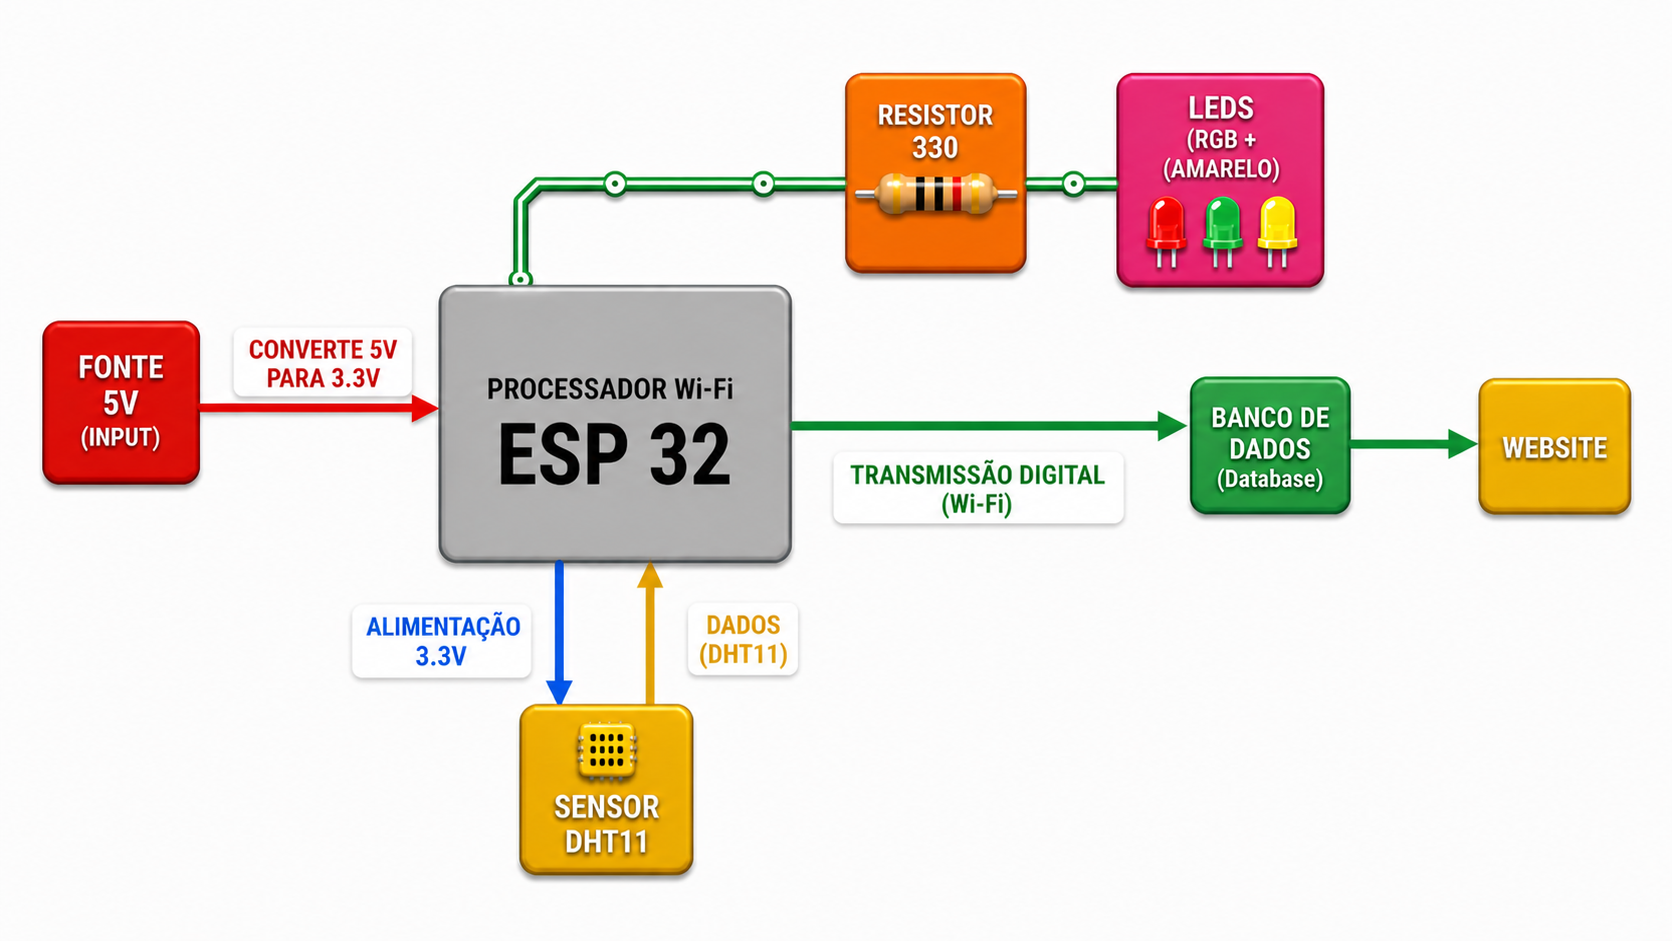
\includegraphics[width=0.7\textwidth]{imagens/diagramaemblocos.png} 
    \caption{Diagrama de blocos do sistema de monitoramento ambiental com ESP32 e DHT11.}
\end{figure}

\subsection{Esquemático Eletrônico}

%texto sobre o esquemático eletronico
As conexões do sensor DHT11 com a ESP32 são: VDD no 3.3V, DATA no pino 15 e GND no GND. Já as conexões dos LEDs com a ESP32 são: LED D1 no pino 32, LED D2 no pino 26, LED D3 no pino 12 no ânodo dos LEDs. No cátodo dos LEDs, todos estão interconectados e se ligam na trilha que vai para o GND da ESP32.

\begin{figure}[H]
   \centering
   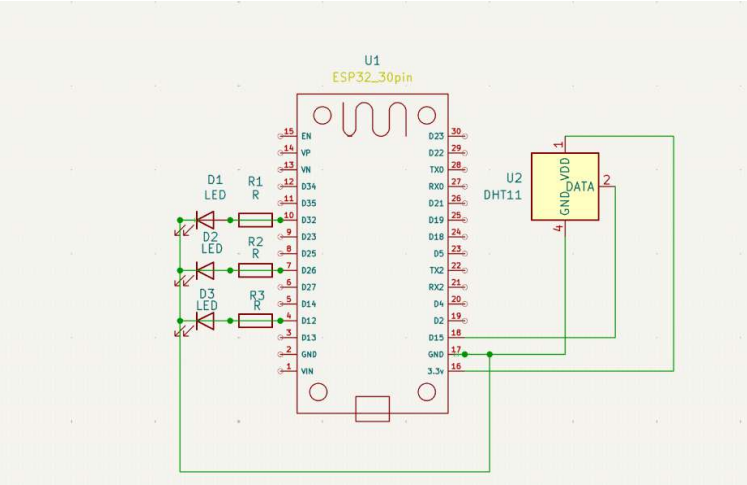
\includegraphics[width=0.7\textwidth]{imagens/esquemático.png} 
    \caption{Esquemático com ESP32 e DHT11.}
\end{figure}

\section{Protótipos de Interface}
\subsection{Protótipo de Baixa Fidelidade}

\begin{figure}[h]
   \centering
   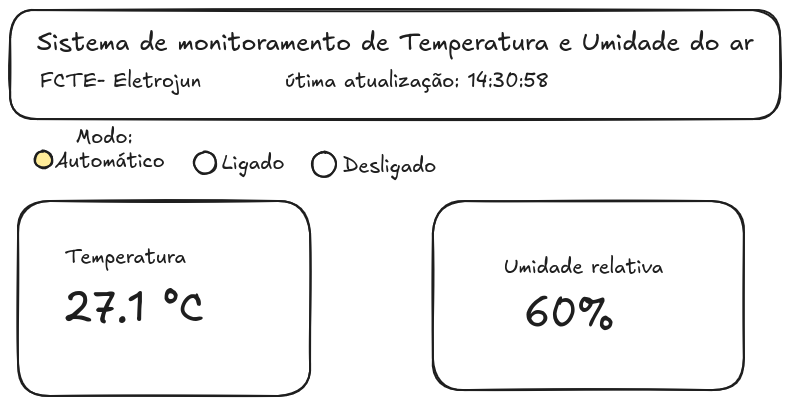
\includegraphics[width=0.8\textwidth]{imagens/Interface_baixa_fidelidade.png} 
    \caption{Protótipo de baixa fidelidade da interface do usuário}
\end{figure}

O protótipo de baixa fidelidade da interface foi desenvolvido com o objetivo de representar a estrutura inicial do sistema de monitoramento de temperatura e umidade do ar. A interface apresenta, de forma simplificada, a organização dos principais elementos necessários para a interação do usuário com o sistema.

Na parte superior, são exibidas informações gerais, como o título do sistema e o horário da última atualização dos dados, permitindo ao usuário identificar rapidamente o estado atual do monitoramento. Logo abaixo, encontra-se a seção de controle de modos de operação, composta pelas opções \textit{Automático}, \textit{Ligado} e \textit{Desligado}, possibilitando a interação direta com o sistema.

A interface também apresenta dois blocos principais de visualização de dados: um destinado à temperatura, exibida em graus Celsius, e outro à umidade relativa do ar, exibida em porcentagem. Esses elementos foram organizados de forma a facilitar a leitura rápida e intuitiva das informações.

O protótipo não contempla aspectos visuais detalhados, como cores definitivas ou estilização avançada, focando apenas na disposição dos componentes e na usabilidade. Dessa forma, ele permite validar a coerência entre a interface proposta e os requisitos funcionais definidos, especialmente aqueles relacionados ao monitoramento em tempo real e ao controle dos modos de operação via interface web.

\subsection{Protótipo de Alta Fidelidade}

\begin{figure}[H]
   \centering
   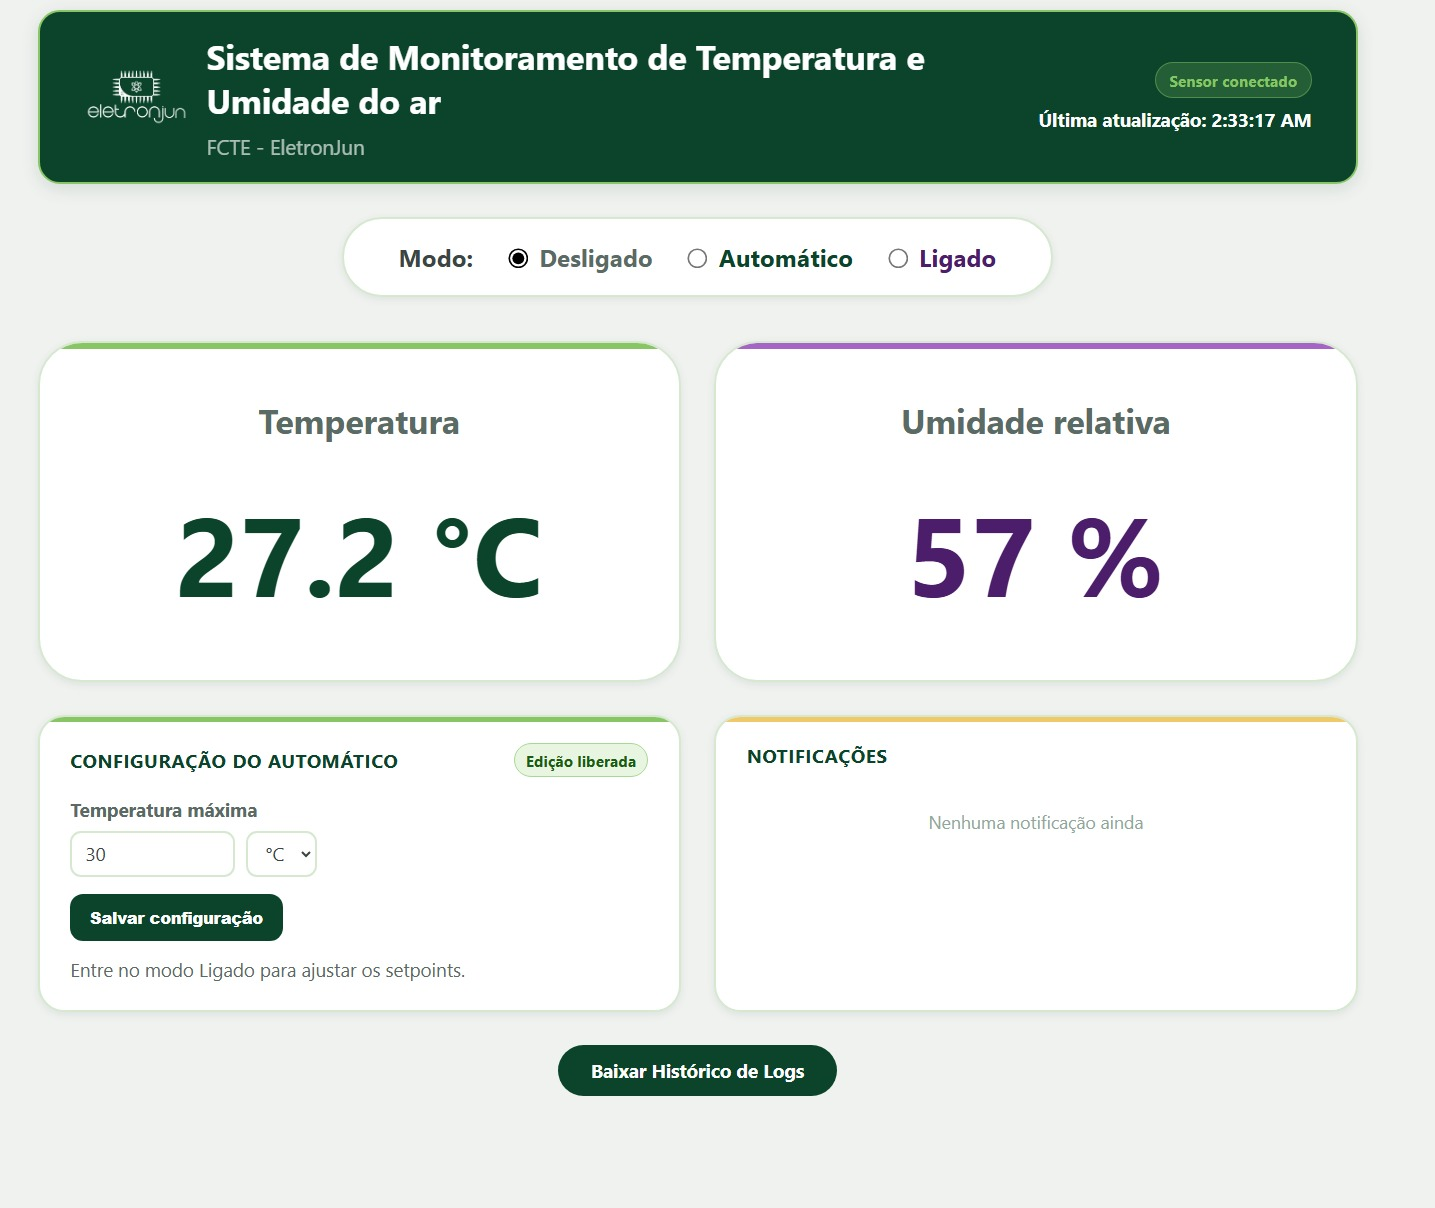
\includegraphics[width=0.5\textwidth]{imagens/sistema_celsius.jpeg} 
    \caption{Protótipo de alta fidelidade da interface do usuário (versão Celsius)}
\end{figure}

\begin{figure}[H]
   \centering
   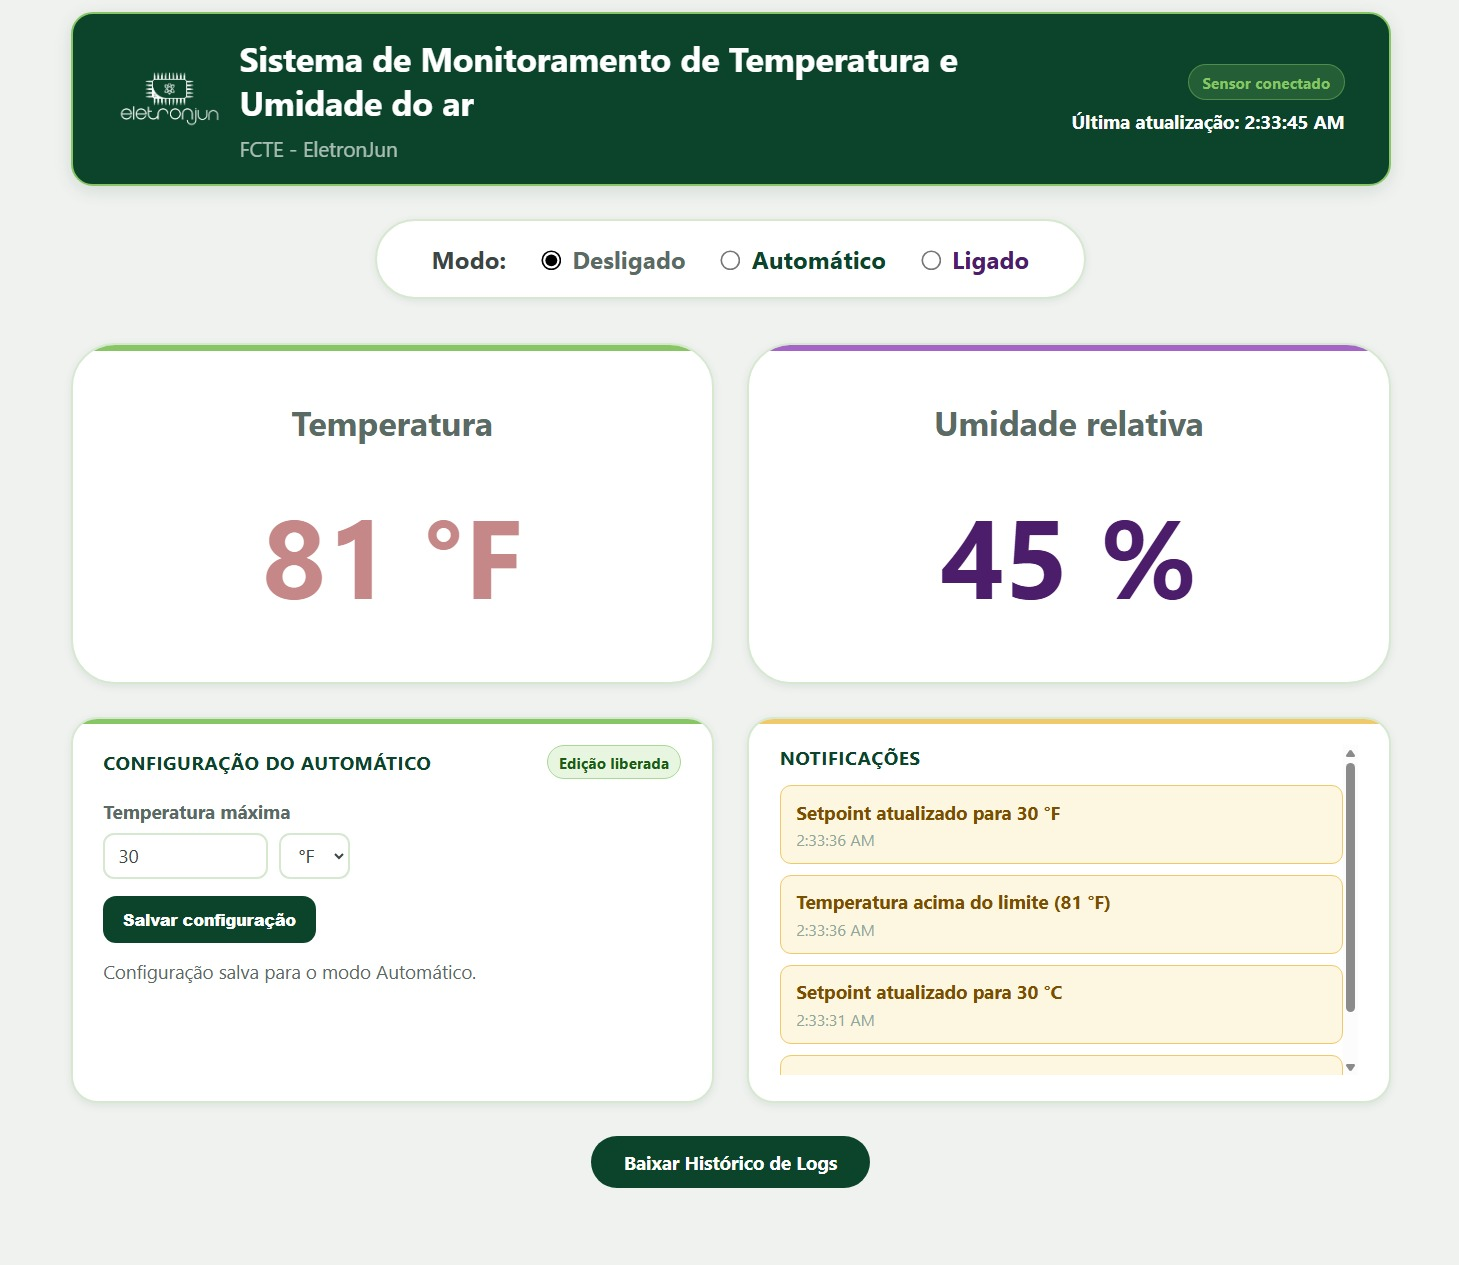
\includegraphics[width=0.5\textwidth]{imagens/sistema_f.jpeg} 
    \caption{Protótipo de alta fidelidade da interface do usuário (versão Fahrenheit)}
\end{figure}

O protótipo de alta fidelidade da interface foi desenvolvido com o objetivo de melhoria e implementação do requisito de hitórico de temperaturas. A interface apresenta, de forma sofisticada, a organização de todos os elementos necessários para a utilização do sistema pelo usuário.

Na parte superior, temos o cabeçalho seguido de informações gerais sobre o projeto, como o título do sistema e o horário da última atualização de temperatura, permitindo o usuário ter conhecimento das informações adquiridas. Abaixo, se encontra a seção de automatização de operação, com as opções \textit{Automático}, \textit{Ligado} e \textit{Desligado}, realizando assim as interações com o sistema.

A interface também apresenta quatro blocos: um para registrar as medições de temperatura, exibida em graus Celsius ou graus Fahrenheit, outro para representar a umidade relativa do ar, exibida em porcentagem, outro para descrever o índice de calor, que realiza uma média do registro das temperaturas, e o último que se trata de um gráfico que mostra a variação das temperaturas e ao lado existe uma parte de alertas, onde o sistema alerta quando a temperatura passa de 28°C. 

Na parte inferior, temos um botão que gera o Histórico de Logs, em um arquivo de texto (.txt), para que o usuário tenha registrado todas as mudanças de temperatura que o sensor registrou.

O protótipo de alta fidelidade passou por melhorias, como a implementação de aspectos visuais, como as cores, a temperatura que quando passa de 28°C o texto pisca, indicando que passou do limite estabelecido, também se tornou funcional os botões de operação, que antes eram apenas esboço do protótipo, e foi realizada a conexão hardware-software, permitindo medições reais de temperatura.


\section{Descrição de Hardware}
\input{Seções/Descricao de Hardware.tex}

\section{Fluxograma de Software}
\begin{figure}[h]
   \centering
   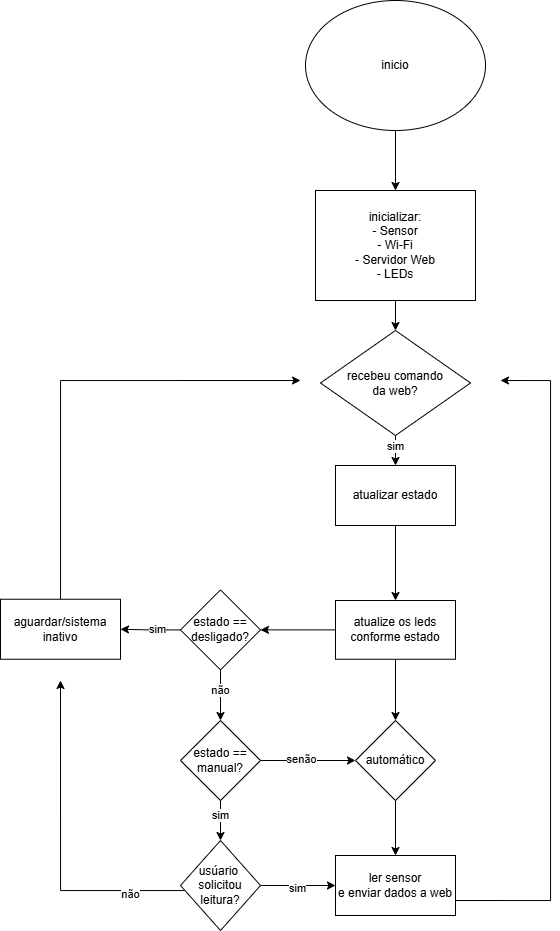
\includegraphics[width=0.6\textwidth]{imagens/fluxograma2.png} 
    \caption{Fluxograma do software do leitor de temperatura}
    \label{fig:fluxograma_software}
\end{figure}

\subsection{Descrição do Fluxograma do Software}

O fluxograma desenvolvido representa a lógica de funcionamento do software embarcado responsável pelo monitoramento de temperatura e umidade, bem como a interação com a interface web e o controle dos LEDs indicadores de estado.

Inicialmente, o sistema realiza a etapa de inicialização, na qual são configurados todos os periféricos necessários para o funcionamento do projeto. Nessa etapa, são inicializados o sensor de temperatura e umidade, o módulo de comunicação Wi-Fi, o servidor web responsável pela interface com o usuário e os pinos de controle dos LEDs. Após a inicialização, o sistema define seu estado inicial como \textbf{Desligado}.

Em seguida, o sistema entra em um \textbf{loop principal de execução contínua}, característica fundamental de sistemas embarcados. Nesse loop, todas as operações do sistema são realizadas de forma cíclica e ininterrupta.

A cada iteração do loop, o sistema verifica se há novos comandos provenientes da interface web. Caso um comando seja recebido, o estado do sistema é atualizado de acordo com a solicitação do usuário, permitindo a alternância entre os modos de operação: Desligado, Manual e Automático. Caso não haja comando, o sistema mantém o estado atual.

Após a possível atualização do estado, os LEDs indicadores são atualizados para refletir o modo de operação vigente, fornecendo uma indicação visual clara do estado do sistema.

\begin{itemize}
\item \textbf{Modo Desligado:}
Neste estado, o sistema permanece inativo, não realizando leituras do sensor nem enviando dados para a interface web. O sistema apenas mantém o loop ativo, aguardando novos comandos do usuário.

\item \textbf{Modo Manual:}  
No modo manual, o sistema aguarda uma solicitação explícita do usuário para realizar a leitura dos dados. Caso o usuário solicite a leitura por meio da interface web, o sistema realiza a coleta dos dados do sensor e os envia para exibição. Caso contrário, permanece em espera, sem executar novas leituras.

\item \textbf{Modo Automático:}  
Neste modo, o sistema realiza leituras periódicas do sensor de forma contínua e automática. Após cada leitura, os dados de temperatura e umidade são enviados à interface web. Um intervalo de tempo é aplicado entre as leituras para evitar sobrecarga do sistema e garantir estabilidade na aquisição dos dados.

\end{itemize}

Independentemente do modo de operação, ao final de cada ciclo de execução, o sistema retorna ao início do loop principal, reiniciando o processo de verificação de comandos e execução das ações correspondentes. Esse comportamento garante a operação contínua e responsiva do sistema.

Dessa forma, o fluxograma representa de maneira clara e estruturada o funcionamento do software, evidenciando a separação entre inicialização, controle de estados, interação com o usuário e execução das funcionalidades principais do sistema.

\section{Descrição de Software}
 A Interface do Usuário (UI) é responsável pela interação direta entre o operador e o sistema. Implementada como uma aplicação web responsiva, ela apresenta em tempo real os valores de temperatura e umidade coletados, disponibiliza os controles para alternância entre os modos de operação (Ligado, Desligado e Automático) e exibe alertas visuais quando os limites pré-estabelecidos são ultrapassados. A interface comunica-se com o firmware do ESP32 por meio de requisições HTTP, enviando comandos e recebendo respostas no formato JSON.

O Controle de Dados é a camada responsável por receber os dados brutos provenientes do sensor DHT11, validá-los, aplicar os procedimentos de calibração necessários e encaminhá-los às demais camadas do sistema. Essa camada implementa também a lógica de detecção de anomalias: quando um valor lido excede os limiares pré-configurados pelo usuário, o módulo aciona simultaneamente a camada de comunicação para enviar notificações por e-mail e a interface web para a exibição dos alertas e da alternância de modos.

A camada de Comunicação gerencia toda a troca de informações entre o hardware e os serviços externos. O firmware do ESP32 utiliza o protocolo HTTP/HTTPS para enviar leituras ao banco de dados remoto e para receber comandos originados na interface web.

Por fim, o Armazenamento de Dados engloba dois mecanismos complementares: o registro remoto em banco de dados relacional, acessado pela interface web para a exibição do histórico de leituras (requisito \textbf{RF06}), e o armazenamento local em arquivo \texttt{.txt} gravado na memória flash do ESP32, que garante a persistência dos dados mesmo na ausência de conectividade com a rede (requisito \textbf{RF09}).

\subsection{Descrição de Alto Nível}

\subsection{Protótipo Funcional}

\subsection{Fluxo de Dados}

O fluxo de operações do sistema pode ser descrito conforme os passos a seguir:

\begin{enumerate}

    \item O ESP32 inicializa, conecta-se à rede Wi-Fi e aguarda comandos ou eventos;
    
    \item O sensor DHT11 realiza medições periódicas de temperatura e umidade, enviando os dados ao ESP32;
    
    \item O ESP32 processa os dados recebidos e os encaminha ao banco de dados via requisição HTTP/HTTPS, registrando cada leitura;

    \item A interface web consulta o banco de dados e exibe os dados de temperatura e umidade em tempo real para o cliente, além de permitir a alternância entre os modos de operação (normal e economia de energia);

    \item Ao receber um comando de alternância de modo, o ESP32 atualiza o estado interno e aciona o LED indicador correspondente, refletindo o modo de operação ativo. 

\end{enumerate}

\section{Bill of Materials}
A tabela a seguir apresenta a lista de materiais (\textit{Bill of Materials} -- BOM) com todos os componentes necessários para a montagem do protótipo, incluindo quantidades e faixas de
preço estimadas para o mercado nacional.

\begin{table}[H]
\centering
\begin{tabularx}{\textwidth}{
    >{\centering\arraybackslash}p{0.55cm}
    X
    >{\centering\arraybackslash}p{2.0cm}
    >{\centering\arraybackslash}p{2.8cm}}
\hline
\rowcolor[HTML]{92D050}
\textbf{N°} & \textbf{Componente} & \textbf{Qtd.} & \textbf{Valor (R\$)} \\
\hline
1  & Microcontrolador Wi-Fi ESP32 (NodeMCU) -- 30 pinos & 1 & 25,00 -- 45,00 \\
\rowcolor[gray]{0.92}
2  & Sensor de Temperatura e Umidade DHT11 & 1 & 6,99 -- 21,89 \\
3  & LED 5\,mm Azul & 3 & 0,41 \\
\rowcolor[gray]{0.92}
4  & Resistor 330\,$\Omega$, 1/4\,W (limitador de corrente dos LEDs) & 4 & 0,30 \\
5  & Placa Fenolite Perfurada (5\,cm $\times$ 7\,cm) & 1 & 2,38 -- 4,90 \\
\rowcolor[gray]{0.92}
6  & Jumper Macho/Macho 10\,cm & 3 & 0,15 -- 0,50 \\
7 & Bateria Alcalina 9\,V (alternativa à fonte) & 1 & 25,00 \\
8 & Adaptador de Bateria 9\,V com Plug P4 & 1 & 2,50 \\
\rowcolor[gray]{0.92}
9 & Cabo Micro-USB para programação / alimentação & 1 & 5,00 -- 10,00 \\
\hline
\multicolumn{3}{r}{\textbf{Valor Total Estimado ( configuração com fonte)}}
& \textbf{R\$\,69,75 -- R\$\,113,22} \\
\hline
\end{tabularx}
\caption{Bill of Materials -- Sistema Leitor de Temperatura e Umidade Ambiente}
\end{table}

\subsection{Total}

O custo total estimado para a montagem de uma unidade do protótipo varia entre \textbf{R\$\,69,75} e \textbf{R\$\,113,22} (com fonte de alimentação), considerando os preços médios praticados no mercado nacional.
\end{document}
